\documentclass[a4paper,12pt]{article}
\usepackage[T1]{fontenc}
\usepackage{imakeidx}
\usepackage{graphicx}
\begin{document}
\tableofcontents

\section{Introduction}
In this document,we spend some words on policies in IT \index{policies}, what is a policy, why we have them, and how many 

\clearpage

\section{What is a policy?}
A policy is a defined set of \emph{targets} every emploee in a \emph{company} has to try to achieve. Evidences proving the efforts to achieve the \emph{target} will be then recorded in some sort of document stored in a place every employee must be aware of. It's considered to be a \emph{statement of intent}. It is a commitment for every employee. The way to abide by the rules of a policy is essentially by showing one is doing the best possible to achieve the \emph{targets}. In every day practice it means spending reasonable effort to show the \emph{target} specified has been fairly achieved. You can label it they way you want and spend hours talking about it but it is essentially \textbf{common sense} written down black and white.
Every employee must be given a \emph{handbook} showing all the policies the company has to comply with.

\section{why we have them?}

Let's take for instance Environmental policies. The reason why we have them is because we might need to be able to deal with Minstery of Defence. Let's say one day a random employee, say \textbf{Giuseppe Mauro Maietta}, all of a sudden is being questioned by Ministery of Defence inspectors who went to check the company is really respecting the policies they have to abide with. If the employee knows what the policies are all about and knows where are they being kept then you have a happy ending, otherwise both the employer and the unlucky \textbf{Giuseppe Mauro Maietta} could be slapped with a huge fine. None of them will be happy, especially \textbf{Giuseppe} when eventually he will face prosecution with all unfortunate consequences. 

It's much better to know where the document is and what the policy is stating. That'll spare you from having to watch \textbf{Giuseppe} doing all sorts of gestures, shouting since he's perfectly aware he's going to get fired anyway.

People down there in Italy, they do all sort of things. You never know what to expect from them so knowing what a policy is, where is being kept is very much crucial indeed  


\section{Type of policies}
\subsection{Acceptable Use Policy}
Defines what is considered to be \emph{acceptable} when it comes to use of equipment and computing services, and the appropriate employee security measures to protect the organization’s corporate resources and proprietary information.
Essentially when you turn the screen of your computer on, you don't want them to spot you while watching porn or sharing confidential information. Porn is easy to manage. You just have to stay away from it. But when you get questioned by an outsider who's not in possession of enough privileges to raise that question, the answer you might want to give is : \emph{I don't know. I'll let you speak with the director if that's ok for you}. It's so simple

\subsection{Environmental policies}
This is a set of sort of good behaviours to follow to make sure the environment is respected. A company that wants to comply to these policies will have to have a saved set of records showing how much fuel are the trucks using and how much is the distance the trucks are covering. The problem is what the company is entitled to do might not always respect real scenario since what we can do is just see on google maps which one is the most convenient road for a truck to take but we cannot guarantee the truck really did that road. It's just to show we're doing what we need to protect the environment

\subsection{Disaster Recover Plan Policy}
Defines the requirement for a baseline disaster recovery plan to be developed and implemented by the company, which describes the process to recover IT Systems, Applications and Data from any type of disaster that causes a major outage. The reason why you need this is just in case you have a real disaster and want to claim for some government support. Eventually you'll get the support but only if you tick all the boxes when they'll investigate on you going through the whole checklist of your own policies you were meant to follow. If you don't have them at all you'll get prosecuted. If you have them but they find out you didn't follow even just one of them they'll have sufficient ground to say "it's your fault if you're not following your own policies what can we do?"

\subsection{Password Protection Policy}
Defines the standard for the creation of strong passwords, the protection of those passwords, and the frequency of change.If you want to break this policy what you can do, if you're right handed, write on your left hand

\[ my \quad password \quad is \quad abacus \]

With a very poor dictionary attack one can log in and do what they want. It's going to look like you did it. And this is because you're a genious: you wrote down the password in a place where everybody can look, and the password itself 
is one of the first words appearing in most English dictionaries. Not a good idea at all


\subsection{Software Installation Policy}
Defines the requirements around installation of third party software on company owned devices.

Allowing employees to install software on company computing devices opens the organization up to unnecessary exposure.  Conflicting file versions or DLLs which can prevent programs from running giving you a very bad day, the introduction of malware from infected installation software, unlicensed software which could be discovered during audit, and programs which can be used to hack the organization’s network are examples of the problems that can be introduced when employees install software on company equipment.

That's why you have to be very strict on the software employees can install, unless troubles are you secret hobby, you are addicted to them and you just can't help


\subsection{Server Security Policy}

Defines \emph{standards} for minimal security configuration for servers inside the organization’s production network, or used in a production capacity.

The purpose of this policy is to define \emph{standards} for the base configuration of internal server equipment that is owned buy the company. Adhering to this policy will minimize unauthorized access and all unfortunate consequences this event might bring
 
\clearpage
\printindex

\section{Some pieces of story}
\subsection{Sony Playstation Network Hacking}

Sony was attacked in the past and did warn that the names, addresses and other personal data of about 77 million people with accounts on its PlayStation Network (PSN) have been stolen.

Gamers have been locked out of the network for a week, but the company took one week to realize what was happening

Sony said it discovered that between 17 and 19 April an "illegal and unauthorised person" got access to people's names, addresses, email address, birthdates, usernames, passwords, logins, security questions and more. The PSN has been shutted down and players who were regular at Monster Hunter had to take a long break before they could face enemies like this again:

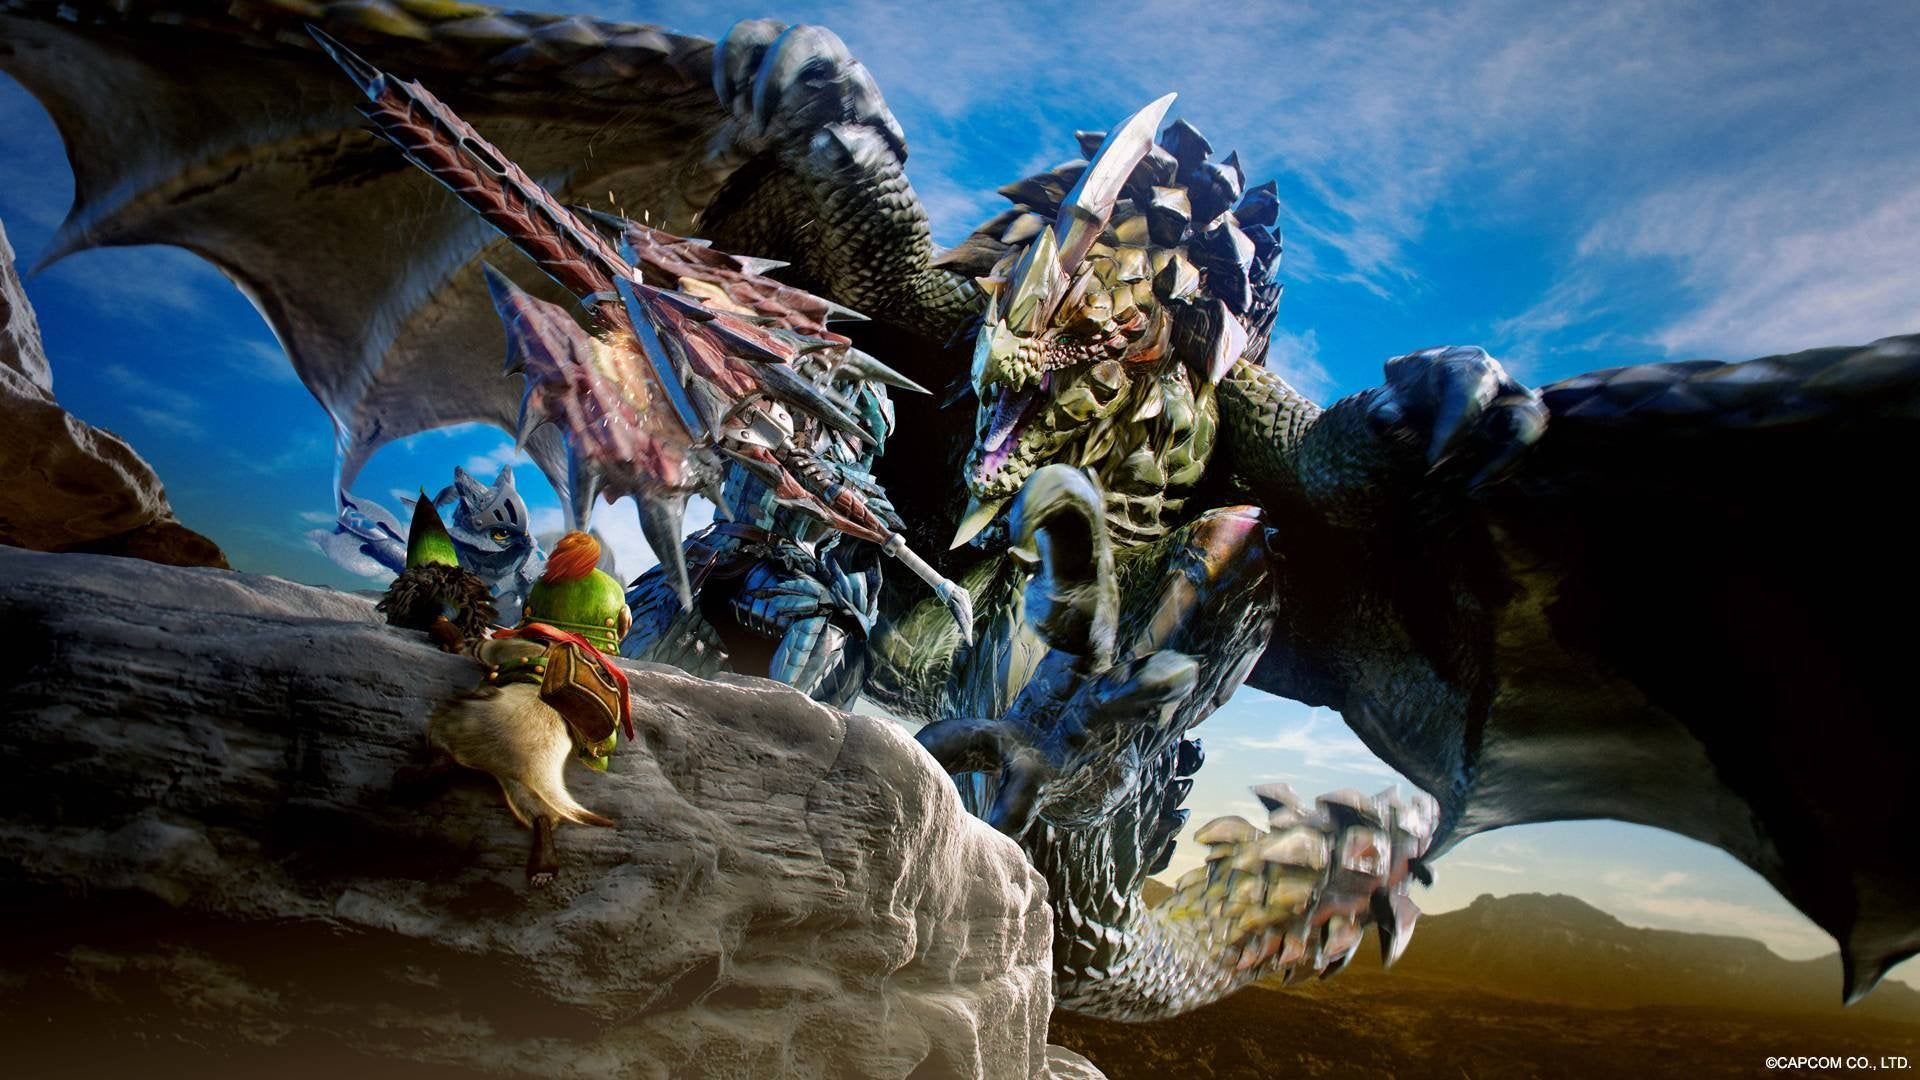
\includegraphics[width=15cm]{./seregios.jpg}

All gamers have been asked to sign lots of paperwork for free after which they have been rewarded with 3 games for free

But Sony upgraded its systems , announced it would finally introduce two-step verification, three years after Microsoft did the same for Xbox Live. There have been no widespread \emph{security breaches} since, although console networks remain vulnerable to concerted DDOS attacks - as seen when both PSN and Xbox Live failed over Christmas 2014.


\end{document}
